\section{Hacking Ratio}
\label{ap:hacking_ratio}
We analyze the changes in the hacking ratio during training for \kernel-14B on the Kernelbench level-2 subset. With the hacking check in \env{}, the hacking ratio steadily decreases from approximately 20\% at the start to around 3\%. We also examine the hacking ratio on the Kernelbench level-1 subset; compared to AutoTriton, which exhibits a hacking ratio of around 10\%, \kernel-14B experiences hacking in only 1.7\% of cases.

\begin{figure*}[htbp]
  \centering
  % Row 1
  \begin{minipage}[t]{0.49\textwidth}
    \centering
    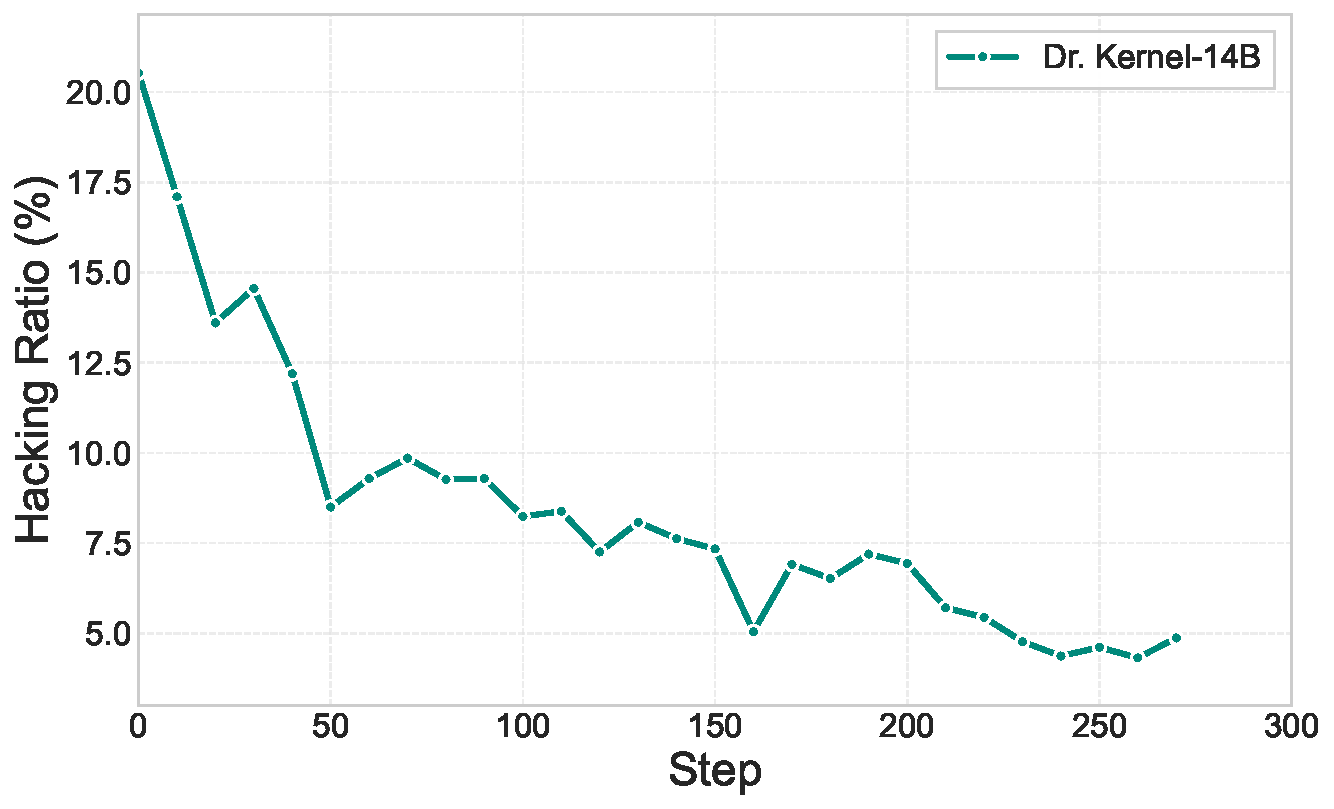
\includegraphics[width=\linewidth]{figures/hacking_ratio/14b_hacking_ratio.pdf}
  \end{minipage}

  \caption{The hacking ratio of \kernel-14B. With the hacking check in \env{}, the hacking ratio decreases from approximately 20\% at the start to only around 3\% in the Kernelbench level-2 subset.}
  \label{fig:hacking-ratio}
\end{figure*}
